\section{Discussion}

In these days software is used every where and seems as it is all about getting data into the data base, pulling it from the data base, sending it elsewhere for profit or fun.

if attackers can infiltrate the SQL that is used for communicating with the data base, then everything will be belongs to them. and if the attacker use SQL query to change authentication query logic they would easily bypass the security. and modify the queries to steal, change or corrupt the data .
in the past SQL Injection was responsible for compromises of many high-profile  organisations (e.g Sony pictures, PBS, MySQL.com) . 
\cite{discussion}
Before we talk about SQL injection I would like to elaborate on SQL it self how it works.

\subsection{What is SQL}
Structured Query Language (SQL) is designed to access and manipulate databases.
it can do the following operations:
\begin{itemize}
\item Execute queries against a database
\item Retrieve data from a database
\item Insert records in a database
\item Update records in a database
\item Delete records in a database
\item Create new databases
\item Create new tables in a database
\item Create stored procedures in a database
\item Create views in a database
\item Set permissions on tables, procedures and views
\end{itemize}
\cite{SQL}


\subsection{ SQL Injection }
Since SQL is used to display data on web page and it let web user to input their own search values.
SQL Injection is a method/technique that malicious users can inject SQL command/queries into an SQL statement via web page input.
\cite{SQLInjection}

\subsection{Exploit Vulnerability}
To better understand how to exploit vulnerability by using SQL Injection technique. 

I used a local web site on my own computer. this web site is based on SAP.NET and SQL Server and it has a database with 3 tables.


\begin{figure}[h!]
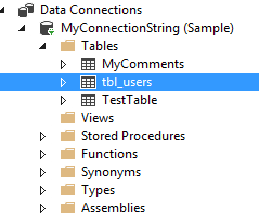
\includegraphics[width=0.4\textwidth]{tblist}
\caption{List of tables in the database }
\end{figure}

The use table is used to store user informations.

\begin{figure}[h!]
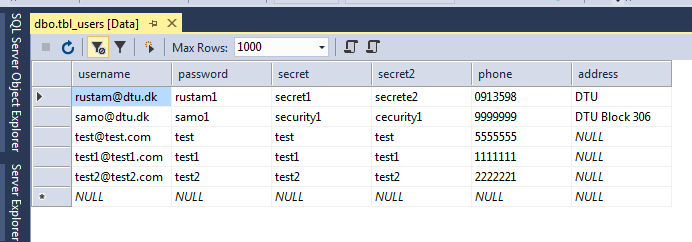
\includegraphics[width=0.8\textwidth]{tbluser}
\caption{User Table}
\end{figure}

MyComments Table is used for storing user comments.

\begin{figure}[h!]
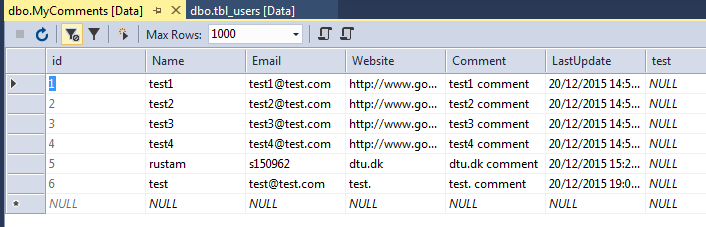
\includegraphics[width=0.8\textwidth]{tblmycomments}
\caption{MyComments Table}
\end{figure}

and the Test table which is not that important.



\subsection{How to Exploit Vulnerability}

As it was explained earlier SQL Injection is insertion of SQL query via input data from a malicious user to an application that is latter passed to instance of SQL server for parsing and execution. 

in this project I will be using UNION based SQL Injection statement.

first we will to go web site which in our case it is a local page using port 1234 which is noting special about this port it is auto generated by visual studio we could use easily replace that port.

\begin{figure}[h!]
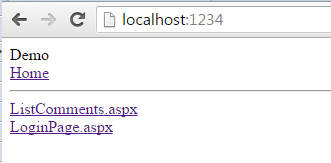
\includegraphics[width=0.4\textwidth]{homepage}
\caption{Home Page}
\end{figure}

Fist we use Union statement to mine all tables name in the database.

the two hyphens "--" represent the SQL comments anything after thse "--" hyphens will not be evaluated by SQL server. 

\begin{figure}[h!]
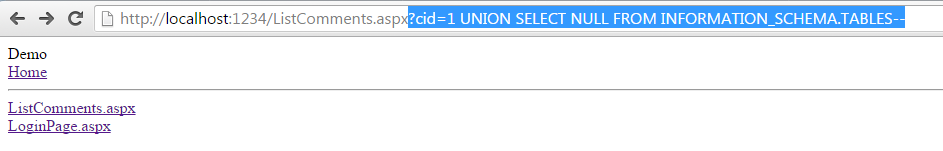
\includegraphics[width=1.0\textwidth]{1sqlinjection}
\caption{First SQL Injection attack}
\end{figure}

it returns the results "all queries combined using a UNION, INTERSECT, or EXCEPT operation must have equal number of expression in their target lists." we get this error when ever we try to run a UNION, INTERSECT or EXCEPT query that has not an equal number of expressions in it SELECT list section. 

\cite{sqllisting2}

\begin{figure}[h!]
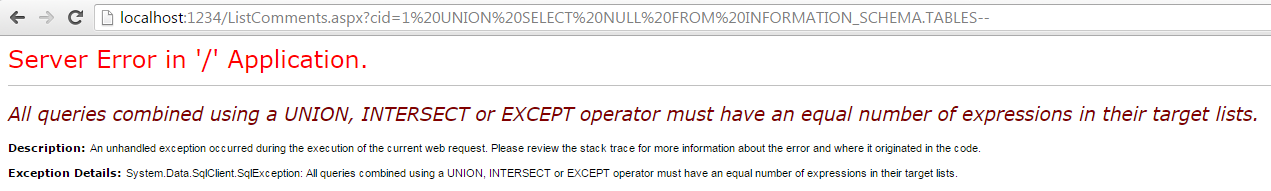
\includegraphics[width=1.0\textwidth]{1sqlinjectionresult}
\caption{First SQL Injection Result}
\end{figure}

we will keep adding NULL expression in the url until the error message disappear.

\begin{figure}[h!]
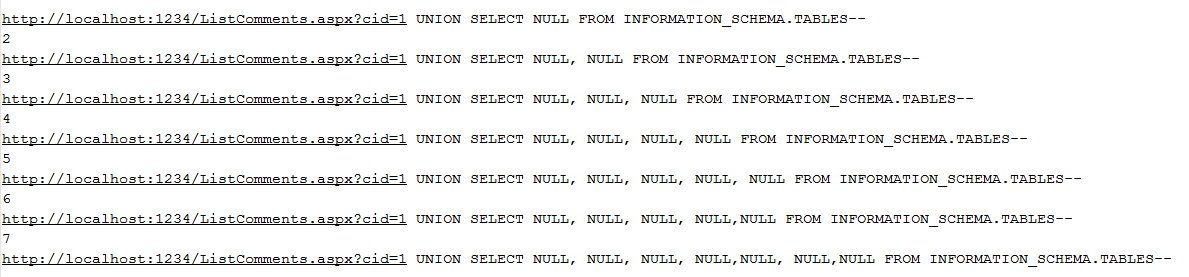
\includegraphics[width=1.0\textwidth]{addnulls}
\caption{Adding NULL to URL}
\end{figure}

once the the query has the equal number of expression in the UNION query the error message will disappear and the first comment will be shown as figure below.

\begin{figure}[h!]
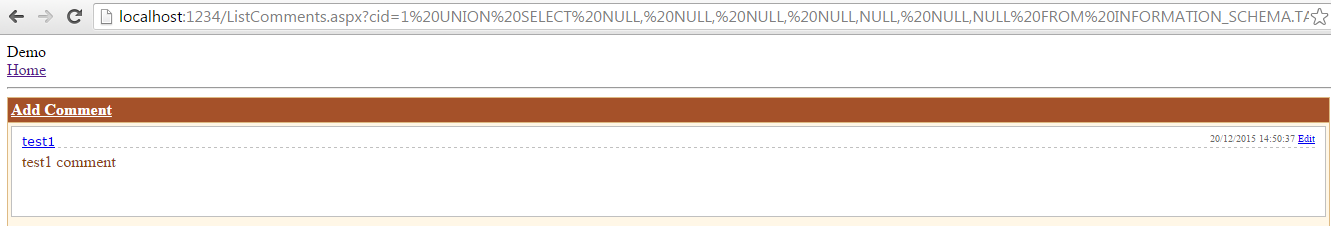
\includegraphics[width=1.0\textwidth]{1comment}
\caption{when error disappear}
\end{figure}

Next we use the same process as before but this time we replace the NULL expression with TABLE NAME to find out how many tables are in the database for further manipulation.

\begin{figure}[h!]
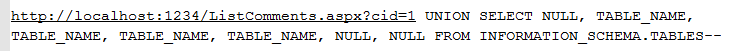
\includegraphics[width=1.0\textwidth]{tablelist}
\caption{SQL Injection to get name of tables in the database}
\end{figure}
as we can see from the figure bellow it shows all the tables in the database.
\begin{figure}[h!]
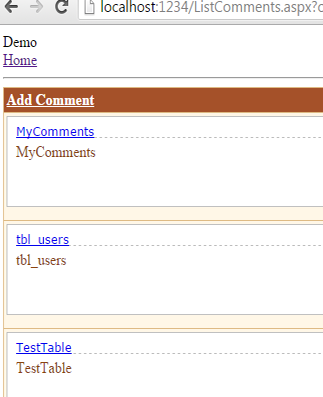
\includegraphics[width=1.0\textwidth]{tlr}
\caption{SQL Injection to get name of tables in the database}
\end{figure}

\begin{figure}[h!]
	\includegraphics[width=0.9\textwidth]{}
	\caption{Result of the SQL injection to show tables}
\end{figure}

now we know the tables in the database and will exploit and attack on user table columns.

\begin{figure}[h!]
	\includegraphics[width=1.0\textwidth]{}
	\caption{SQL Injection to get user table columns}
\end{figure}

the result shows what column used in user tables

\begin{figure}[h!]
	\includegraphics[width=0.7\textwidth]{}
	\caption{SQL Injection to get user table columns}
\end{figure}








\subsubsection{sub section 2}
\paragraph{paragraph}
new par this is last par

new back ground